% !TEX encoding = UTF-8 Unicode
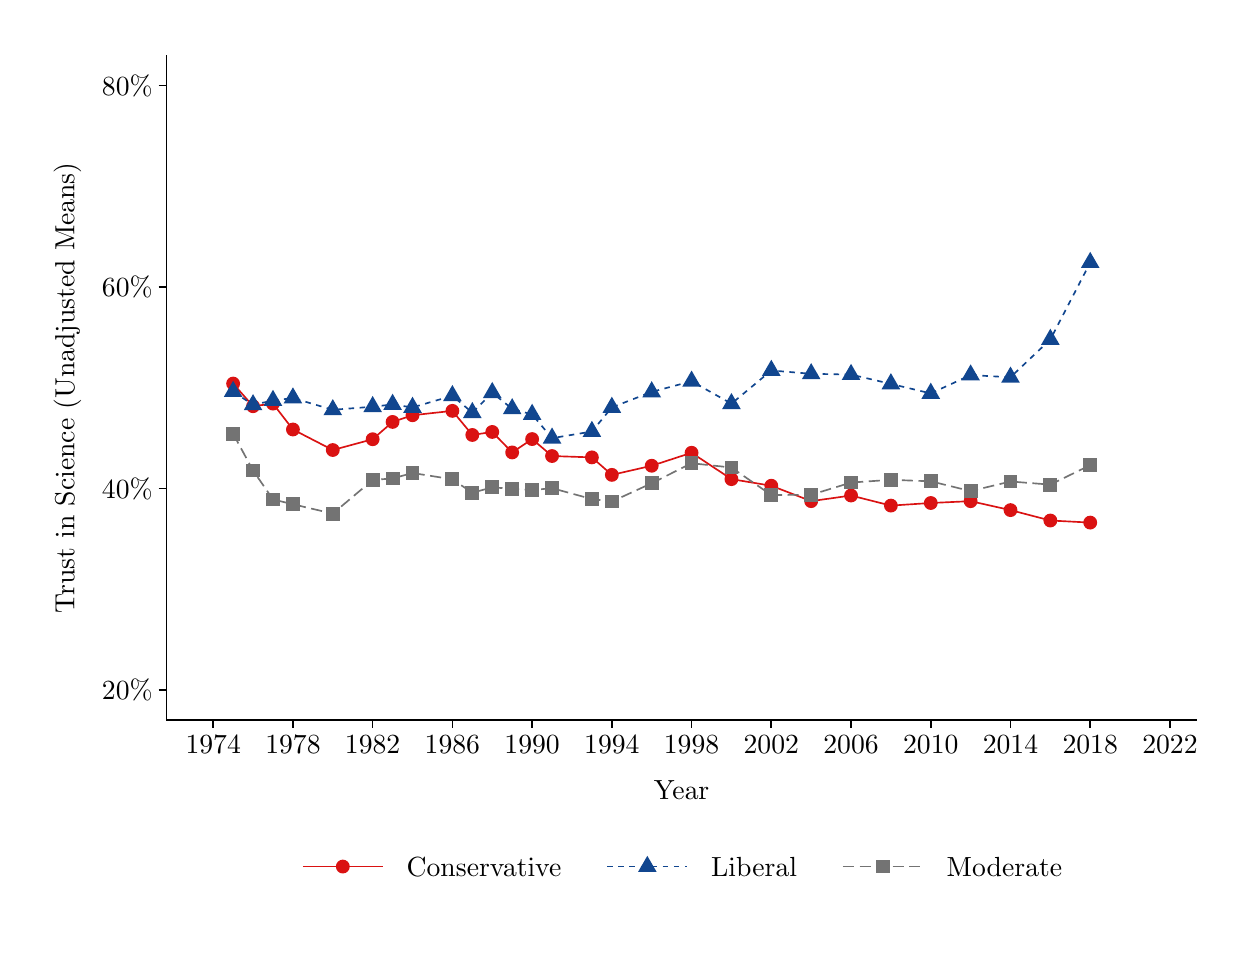
\begin{tikzpicture}[x=1pt,y=1pt]
\definecolor{fillColor}{RGB}{255,255,255}
\path[use as bounding box,fill=fillColor,fill opacity=0.00] (0,0) rectangle (432.48,324.36);
\begin{scope}
\path[clip] (  0.00,  0.00) rectangle (432.48,324.36);
\definecolor{fillColor}{RGB}{255,255,255}

\path[fill=fillColor] ( -0.00,  0.00) rectangle (432.48,324.36);
\end{scope}
\begin{scope}
\path[clip] ( 50.11, 74.07) rectangle (422.48,314.36);
\definecolor{fillColor}{RGB}{255,255,255}

\path[fill=fillColor] ( 50.11, 74.07) rectangle (422.48,314.36);
\definecolor{drawColor}{RGB}{218,18,18}

\path[draw=drawColor,line width= 0.6pt,line join=round] ( 74.24,195.75) --
	( 81.44,187.57) --
	( 88.64,188.51) --
	( 95.85,179.16) --
	(110.25,171.74) --
	(124.66,175.64) --
	(131.86,181.89) --
	(139.06,184.31) --
	(153.47,185.89) --
	(160.67,177.18) --
	(167.87,178.27) --
	(175.07,170.87) --
	(182.28,175.70) --
	(189.48,169.57) --
	(203.88,169.08) --
	(211.09,162.76) --
	(225.49,166.06) --
	(239.90,170.75) --
	(254.30,161.22) --
	(268.71,158.84) --
	(283.11,153.27) --
	(297.52,155.30) --
	(311.92,151.66) --
	(326.33,152.60) --
	(340.73,153.26) --
	(355.14,150.03) --
	(369.54,146.27) --
	(383.95,145.52);
\definecolor{drawColor}{RGB}{17,70,143}

\path[draw=drawColor,line width= 0.6pt,dash pattern=on 2pt off 2pt ,line join=round] ( 74.24,192.87) --
	( 81.44,188.08) --
	( 88.64,189.62) --
	( 95.85,190.52) --
	(110.25,186.27) --
	(124.66,187.39) --
	(131.86,188.20) --
	(139.06,187.13) --
	(153.47,191.36) --
	(160.67,185.24) --
	(167.87,192.46) --
	(175.07,186.62) --
	(182.28,184.58) --
	(189.48,176.03) --
	(203.88,178.43) --
	(211.09,187.14) --
	(225.49,192.74) --
	(239.90,196.59) --
	(254.30,188.48) --
	(268.71,200.49) --
	(283.11,199.28) --
	(297.52,199.00) --
	(311.92,195.64) --
	(326.33,192.20) --
	(340.73,198.82) --
	(355.14,198.03) --
	(369.54,211.69) --
	(383.95,239.47);
\definecolor{drawColor}{gray}{0.45}

\path[draw=drawColor,line width= 0.6pt,dash pattern=on 4pt off 2pt ,line join=round] ( 74.24,177.64) --
	( 81.44,164.34) --
	( 88.64,153.89) --
	( 95.85,152.14) --
	(110.25,148.76) --
	(124.66,160.92) --
	(131.86,161.48) --
	(139.06,163.43) --
	(153.47,161.17) --
	(160.67,156.31) --
	(167.87,158.25) --
	(175.07,157.74) --
	(182.28,157.27) --
	(189.48,157.95) --
	(203.88,154.02) --
	(211.09,153.12) --
	(225.49,159.74) --
	(239.90,166.97) --
	(254.30,165.41) --
	(268.71,155.48) --
	(283.11,155.57) --
	(297.52,159.98) --
	(311.92,160.98) --
	(326.33,160.44) --
	(340.73,156.90) --
	(355.14,160.37) --
	(369.54,159.24) --
	(383.95,166.27);
\definecolor{fillColor}{RGB}{218,18,18}

\path[fill=fillColor] ( 74.24,195.75) circle (  2.50);
\definecolor{fillColor}{RGB}{17,70,143}

\path[fill=fillColor] ( 74.24,196.76) --
	( 77.60,190.93) --
	( 70.87,190.93) --
	cycle;
\definecolor{fillColor}{gray}{0.45}

\path[fill=fillColor] ( 71.74,175.14) --
	( 76.74,175.14) --
	( 76.74,180.13) --
	( 71.74,180.13) --
	cycle;
\definecolor{fillColor}{RGB}{218,18,18}

\path[fill=fillColor] ( 81.44,187.57) circle (  2.50);
\definecolor{fillColor}{RGB}{17,70,143}

\path[fill=fillColor] ( 81.44,191.96) --
	( 84.80,186.14) --
	( 78.08,186.14) --
	cycle;
\definecolor{fillColor}{gray}{0.45}

\path[fill=fillColor] ( 78.94,161.84) --
	( 83.94,161.84) --
	( 83.94,166.84) --
	( 78.94,166.84) --
	cycle;
\definecolor{fillColor}{RGB}{218,18,18}

\path[fill=fillColor] ( 88.64,188.51) circle (  2.50);
\definecolor{fillColor}{RGB}{17,70,143}

\path[fill=fillColor] ( 88.64,193.51) --
	( 92.01,187.68) --
	( 85.28,187.68) --
	cycle;
\definecolor{fillColor}{gray}{0.45}

\path[fill=fillColor] ( 86.15,151.40) --
	( 91.14,151.40) --
	( 91.14,156.39) --
	( 86.15,156.39) --
	cycle;
\definecolor{fillColor}{RGB}{218,18,18}

\path[fill=fillColor] ( 95.85,179.16) circle (  2.50);
\definecolor{fillColor}{RGB}{17,70,143}

\path[fill=fillColor] ( 95.85,194.41) --
	( 99.21,188.58) --
	( 92.48,188.58) --
	cycle;
\definecolor{fillColor}{gray}{0.45}

\path[fill=fillColor] ( 93.35,149.64) --
	( 98.34,149.64) --
	( 98.34,154.64) --
	( 93.35,154.64) --
	cycle;
\definecolor{fillColor}{RGB}{218,18,18}

\path[fill=fillColor] (110.25,171.74) circle (  2.50);
\definecolor{fillColor}{RGB}{17,70,143}

\path[fill=fillColor] (110.25,190.15) --
	(113.62,184.33) --
	(106.89,184.33) --
	cycle;
\definecolor{fillColor}{gray}{0.45}

\path[fill=fillColor] (107.75,146.26) --
	(112.75,146.26) --
	(112.75,151.26) --
	(107.75,151.26) --
	cycle;
\definecolor{fillColor}{RGB}{218,18,18}

\path[fill=fillColor] (124.66,175.64) circle (  2.50);
\definecolor{fillColor}{RGB}{17,70,143}

\path[fill=fillColor] (124.66,191.28) --
	(128.02,185.45) --
	(121.29,185.45) --
	cycle;
\definecolor{fillColor}{gray}{0.45}

\path[fill=fillColor] (122.16,158.43) --
	(127.15,158.43) --
	(127.15,163.42) --
	(122.16,163.42) --
	cycle;
\definecolor{fillColor}{RGB}{218,18,18}

\path[fill=fillColor] (131.86,181.89) circle (  2.50);
\definecolor{fillColor}{RGB}{17,70,143}

\path[fill=fillColor] (131.86,192.09) --
	(135.22,186.26) --
	(128.50,186.26) --
	cycle;
\definecolor{fillColor}{gray}{0.45}

\path[fill=fillColor] (129.36,158.98) --
	(134.36,158.98) --
	(134.36,163.98) --
	(129.36,163.98) --
	cycle;
\definecolor{fillColor}{RGB}{218,18,18}

\path[fill=fillColor] (139.06,184.31) circle (  2.50);
\definecolor{fillColor}{RGB}{17,70,143}

\path[fill=fillColor] (139.06,191.01) --
	(142.43,185.19) --
	(135.70,185.19) --
	cycle;
\definecolor{fillColor}{gray}{0.45}

\path[fill=fillColor] (136.56,160.93) --
	(141.56,160.93) --
	(141.56,165.93) --
	(136.56,165.93) --
	cycle;
\definecolor{fillColor}{RGB}{218,18,18}

\path[fill=fillColor] (153.47,185.89) circle (  2.50);
\definecolor{fillColor}{RGB}{17,70,143}

\path[fill=fillColor] (153.47,195.25) --
	(156.83,189.42) --
	(150.10,189.42) --
	cycle;
\definecolor{fillColor}{gray}{0.45}

\path[fill=fillColor] (150.97,158.67) --
	(155.96,158.67) --
	(155.96,163.66) --
	(150.97,163.66) --
	cycle;
\definecolor{fillColor}{RGB}{218,18,18}

\path[fill=fillColor] (160.67,177.18) circle (  2.50);
\definecolor{fillColor}{RGB}{17,70,143}

\path[fill=fillColor] (160.67,189.12) --
	(164.03,183.29) --
	(157.31,183.29) --
	cycle;
\definecolor{fillColor}{gray}{0.45}

\path[fill=fillColor] (158.17,153.81) --
	(163.17,153.81) --
	(163.17,158.81) --
	(158.17,158.81) --
	cycle;
\definecolor{fillColor}{RGB}{218,18,18}

\path[fill=fillColor] (167.87,178.27) circle (  2.50);
\definecolor{fillColor}{RGB}{17,70,143}

\path[fill=fillColor] (167.87,196.35) --
	(171.24,190.52) --
	(164.51,190.52) --
	cycle;
\definecolor{fillColor}{gray}{0.45}

\path[fill=fillColor] (165.37,155.75) --
	(170.37,155.75) --
	(170.37,160.75) --
	(165.37,160.75) --
	cycle;
\definecolor{fillColor}{RGB}{218,18,18}

\path[fill=fillColor] (175.07,170.87) circle (  2.50);
\definecolor{fillColor}{RGB}{17,70,143}

\path[fill=fillColor] (175.07,190.50) --
	(178.44,184.68) --
	(171.71,184.68) --
	cycle;
\definecolor{fillColor}{gray}{0.45}

\path[fill=fillColor] (172.58,155.24) --
	(177.57,155.24) --
	(177.57,160.24) --
	(172.58,160.24) --
	cycle;
\definecolor{fillColor}{RGB}{218,18,18}

\path[fill=fillColor] (182.28,175.70) circle (  2.50);
\definecolor{fillColor}{RGB}{17,70,143}

\path[fill=fillColor] (182.28,188.47) --
	(185.64,182.64) --
	(178.91,182.64) --
	cycle;
\definecolor{fillColor}{gray}{0.45}

\path[fill=fillColor] (179.78,154.77) --
	(184.77,154.77) --
	(184.77,159.76) --
	(179.78,159.76) --
	cycle;
\definecolor{fillColor}{RGB}{218,18,18}

\path[fill=fillColor] (189.48,169.57) circle (  2.50);
\definecolor{fillColor}{RGB}{17,70,143}

\path[fill=fillColor] (189.48,179.91) --
	(192.84,174.08) --
	(186.12,174.08) --
	cycle;
\definecolor{fillColor}{gray}{0.45}

\path[fill=fillColor] (186.98,155.46) --
	(191.98,155.46) --
	(191.98,160.45) --
	(186.98,160.45) --
	cycle;
\definecolor{fillColor}{RGB}{218,18,18}

\path[fill=fillColor] (203.88,169.08) circle (  2.50);
\definecolor{fillColor}{RGB}{17,70,143}

\path[fill=fillColor] (203.88,182.31) --
	(207.25,176.48) --
	(200.52,176.48) --
	cycle;
\definecolor{fillColor}{gray}{0.45}

\path[fill=fillColor] (201.39,151.52) --
	(206.38,151.52) --
	(206.38,156.52) --
	(201.39,156.52) --
	cycle;
\definecolor{fillColor}{RGB}{218,18,18}

\path[fill=fillColor] (211.09,162.76) circle (  2.50);
\definecolor{fillColor}{RGB}{17,70,143}

\path[fill=fillColor] (211.09,191.02) --
	(214.45,185.20) --
	(207.72,185.20) --
	cycle;
\definecolor{fillColor}{gray}{0.45}

\path[fill=fillColor] (208.59,150.63) --
	(213.58,150.63) --
	(213.58,155.62) --
	(208.59,155.62) --
	cycle;
\definecolor{fillColor}{RGB}{218,18,18}

\path[fill=fillColor] (225.49,166.06) circle (  2.50);
\definecolor{fillColor}{RGB}{17,70,143}

\path[fill=fillColor] (225.49,196.63) --
	(228.86,190.80) --
	(222.13,190.80) --
	cycle;
\definecolor{fillColor}{gray}{0.45}

\path[fill=fillColor] (222.99,157.24) --
	(227.99,157.24) --
	(227.99,162.24) --
	(222.99,162.24) --
	cycle;
\definecolor{fillColor}{RGB}{218,18,18}

\path[fill=fillColor] (239.90,170.75) circle (  2.50);
\definecolor{fillColor}{RGB}{17,70,143}

\path[fill=fillColor] (239.90,200.47) --
	(243.26,194.65) --
	(236.53,194.65) --
	cycle;
\definecolor{fillColor}{gray}{0.45}

\path[fill=fillColor] (237.40,164.47) --
	(242.39,164.47) --
	(242.39,169.46) --
	(237.40,169.46) --
	cycle;
\definecolor{fillColor}{RGB}{218,18,18}

\path[fill=fillColor] (254.30,161.22) circle (  2.50);
\definecolor{fillColor}{RGB}{17,70,143}

\path[fill=fillColor] (254.30,192.36) --
	(257.67,186.54) --
	(250.94,186.54) --
	cycle;
\definecolor{fillColor}{gray}{0.45}

\path[fill=fillColor] (251.80,162.91) --
	(256.80,162.91) --
	(256.80,167.91) --
	(251.80,167.91) --
	cycle;
\definecolor{fillColor}{RGB}{218,18,18}

\path[fill=fillColor] (268.71,158.84) circle (  2.50);
\definecolor{fillColor}{RGB}{17,70,143}

\path[fill=fillColor] (268.71,204.37) --
	(272.07,198.55) --
	(265.34,198.55) --
	cycle;
\definecolor{fillColor}{gray}{0.45}

\path[fill=fillColor] (266.21,152.99) --
	(271.21,152.99) --
	(271.21,157.98) --
	(266.21,157.98) --
	cycle;
\definecolor{fillColor}{RGB}{218,18,18}

\path[fill=fillColor] (283.11,153.27) circle (  2.50);
\definecolor{fillColor}{RGB}{17,70,143}

\path[fill=fillColor] (283.11,203.16) --
	(286.48,197.34) --
	(279.75,197.34) --
	cycle;
\definecolor{fillColor}{gray}{0.45}

\path[fill=fillColor] (280.61,153.07) --
	(285.61,153.07) --
	(285.61,158.07) --
	(280.61,158.07) --
	cycle;
\definecolor{fillColor}{RGB}{218,18,18}

\path[fill=fillColor] (297.52,155.30) circle (  2.50);
\definecolor{fillColor}{RGB}{17,70,143}

\path[fill=fillColor] (297.52,202.89) --
	(300.88,197.06) --
	(294.15,197.06) --
	cycle;
\definecolor{fillColor}{gray}{0.45}

\path[fill=fillColor] (295.02,157.48) --
	(300.02,157.48) --
	(300.02,162.48) --
	(295.02,162.48) --
	cycle;
\definecolor{fillColor}{RGB}{218,18,18}

\path[fill=fillColor] (311.92,151.66) circle (  2.50);
\definecolor{fillColor}{RGB}{17,70,143}

\path[fill=fillColor] (311.92,199.53) --
	(315.29,193.70) --
	(308.56,193.70) --
	cycle;
\definecolor{fillColor}{gray}{0.45}

\path[fill=fillColor] (309.43,158.49) --
	(314.42,158.49) --
	(314.42,163.48) --
	(309.43,163.48) --
	cycle;
\definecolor{fillColor}{RGB}{218,18,18}

\path[fill=fillColor] (326.33,152.60) circle (  2.50);
\definecolor{fillColor}{RGB}{17,70,143}

\path[fill=fillColor] (326.33,196.08) --
	(329.69,190.25) --
	(322.96,190.25) --
	cycle;
\definecolor{fillColor}{gray}{0.45}

\path[fill=fillColor] (323.83,157.94) --
	(328.83,157.94) --
	(328.83,162.94) --
	(323.83,162.94) --
	cycle;
\definecolor{fillColor}{RGB}{218,18,18}

\path[fill=fillColor] (340.73,153.26) circle (  2.50);
\definecolor{fillColor}{RGB}{17,70,143}

\path[fill=fillColor] (340.73,202.71) --
	(344.10,196.88) --
	(337.37,196.88) --
	cycle;
\definecolor{fillColor}{gray}{0.45}

\path[fill=fillColor] (338.24,154.41) --
	(343.23,154.41) --
	(343.23,159.40) --
	(338.24,159.40) --
	cycle;
\definecolor{fillColor}{RGB}{218,18,18}

\path[fill=fillColor] (355.14,150.03) circle (  2.50);
\definecolor{fillColor}{RGB}{17,70,143}

\path[fill=fillColor] (355.14,201.92) --
	(358.50,196.09) --
	(351.77,196.09) --
	cycle;
\definecolor{fillColor}{gray}{0.45}

\path[fill=fillColor] (352.64,157.87) --
	(357.64,157.87) --
	(357.64,162.86) --
	(352.64,162.86) --
	cycle;
\definecolor{fillColor}{RGB}{218,18,18}

\path[fill=fillColor] (369.54,146.27) circle (  2.50);
\definecolor{fillColor}{RGB}{17,70,143}

\path[fill=fillColor] (369.54,215.58) --
	(372.91,209.75) --
	(366.18,209.75) --
	cycle;
\definecolor{fillColor}{gray}{0.45}

\path[fill=fillColor] (367.05,156.75) --
	(372.04,156.75) --
	(372.04,161.74) --
	(367.05,161.74) --
	cycle;
\definecolor{fillColor}{RGB}{218,18,18}

\path[fill=fillColor] (383.95,145.52) circle (  2.50);
\definecolor{fillColor}{RGB}{17,70,143}

\path[fill=fillColor] (383.95,243.36) --
	(387.31,237.53) --
	(380.58,237.53) --
	cycle;
\definecolor{fillColor}{gray}{0.45}

\path[fill=fillColor] (381.45,163.78) --
	(386.45,163.78) --
	(386.45,168.77) --
	(381.45,168.77) --
	cycle;
\end{scope}
\begin{scope}
\path[clip] (  0.00,  0.00) rectangle (432.48,324.36);
\definecolor{drawColor}{RGB}{0,0,0}

\path[draw=drawColor,line width= 0.6pt,line join=round] ( 50.11, 74.07) --
	( 50.11,314.36);
\end{scope}
\begin{scope}
\path[clip] (  0.00,  0.00) rectangle (432.48,324.36);
\definecolor{drawColor}{RGB}{0,0,0}

\node[text=drawColor,anchor=base east,inner sep=0pt, outer sep=0pt, scale=  1.00] at ( 45.16, 81.55) {20{\%}};

\node[text=drawColor,anchor=base east,inner sep=0pt, outer sep=0pt, scale=  1.00] at ( 45.16,154.36) {40{\%}};

\node[text=drawColor,anchor=base east,inner sep=0pt, outer sep=0pt, scale=  1.00] at ( 45.16,227.18) {60{\%}};

\node[text=drawColor,anchor=base east,inner sep=0pt, outer sep=0pt, scale=  1.00] at ( 45.16,300.00) {80{\%}};
\end{scope}
\begin{scope}
\path[clip] (  0.00,  0.00) rectangle (432.48,324.36);
\definecolor{drawColor}{RGB}{0,0,0}

\path[draw=drawColor,line width= 0.6pt,line join=round] ( 47.36, 84.99) --
	( 50.11, 84.99);

\path[draw=drawColor,line width= 0.6pt,line join=round] ( 47.36,157.81) --
	( 50.11,157.81);

\path[draw=drawColor,line width= 0.6pt,line join=round] ( 47.36,230.62) --
	( 50.11,230.62);

\path[draw=drawColor,line width= 0.6pt,line join=round] ( 47.36,303.44) --
	( 50.11,303.44);
\end{scope}
\begin{scope}
\path[clip] (  0.00,  0.00) rectangle (432.48,324.36);
\definecolor{drawColor}{RGB}{0,0,0}

\path[draw=drawColor,line width= 0.6pt,line join=round] ( 50.11, 74.07) --
	(422.48, 74.07);
\end{scope}
\begin{scope}
\path[clip] (  0.00,  0.00) rectangle (432.48,324.36);
\definecolor{drawColor}{RGB}{0,0,0}

\path[draw=drawColor,line width= 0.6pt,line join=round] ( 67.04, 71.32) --
	( 67.04, 74.07);

\path[draw=drawColor,line width= 0.6pt,line join=round] ( 95.85, 71.32) --
	( 95.85, 74.07);

\path[draw=drawColor,line width= 0.6pt,line join=round] (124.66, 71.32) --
	(124.66, 74.07);

\path[draw=drawColor,line width= 0.6pt,line join=round] (153.47, 71.32) --
	(153.47, 74.07);

\path[draw=drawColor,line width= 0.6pt,line join=round] (182.28, 71.32) --
	(182.28, 74.07);

\path[draw=drawColor,line width= 0.6pt,line join=round] (211.09, 71.32) --
	(211.09, 74.07);

\path[draw=drawColor,line width= 0.6pt,line join=round] (239.90, 71.32) --
	(239.90, 74.07);

\path[draw=drawColor,line width= 0.6pt,line join=round] (268.71, 71.32) --
	(268.71, 74.07);

\path[draw=drawColor,line width= 0.6pt,line join=round] (297.52, 71.32) --
	(297.52, 74.07);

\path[draw=drawColor,line width= 0.6pt,line join=round] (326.33, 71.32) --
	(326.33, 74.07);

\path[draw=drawColor,line width= 0.6pt,line join=round] (355.14, 71.32) --
	(355.14, 74.07);

\path[draw=drawColor,line width= 0.6pt,line join=round] (383.95, 71.32) --
	(383.95, 74.07);

\path[draw=drawColor,line width= 0.6pt,line join=round] (412.76, 71.32) --
	(412.76, 74.07);
\end{scope}
\begin{scope}
\path[clip] (  0.00,  0.00) rectangle (432.48,324.36);
\definecolor{drawColor}{RGB}{0,0,0}

\node[text=drawColor,anchor=base,inner sep=0pt, outer sep=0pt, scale=  1.00] at ( 67.04, 62.23) {1974};

\node[text=drawColor,anchor=base,inner sep=0pt, outer sep=0pt, scale=  1.00] at ( 95.85, 62.23) {1978};

\node[text=drawColor,anchor=base,inner sep=0pt, outer sep=0pt, scale=  1.00] at (124.66, 62.23) {1982};

\node[text=drawColor,anchor=base,inner sep=0pt, outer sep=0pt, scale=  1.00] at (153.47, 62.23) {1986};

\node[text=drawColor,anchor=base,inner sep=0pt, outer sep=0pt, scale=  1.00] at (182.28, 62.23) {1990};

\node[text=drawColor,anchor=base,inner sep=0pt, outer sep=0pt, scale=  1.00] at (211.09, 62.23) {1994};

\node[text=drawColor,anchor=base,inner sep=0pt, outer sep=0pt, scale=  1.00] at (239.90, 62.23) {1998};

\node[text=drawColor,anchor=base,inner sep=0pt, outer sep=0pt, scale=  1.00] at (268.71, 62.23) {2002};

\node[text=drawColor,anchor=base,inner sep=0pt, outer sep=0pt, scale=  1.00] at (297.52, 62.23) {2006};

\node[text=drawColor,anchor=base,inner sep=0pt, outer sep=0pt, scale=  1.00] at (326.33, 62.23) {2010};

\node[text=drawColor,anchor=base,inner sep=0pt, outer sep=0pt, scale=  1.00] at (355.14, 62.23) {2014};

\node[text=drawColor,anchor=base,inner sep=0pt, outer sep=0pt, scale=  1.00] at (383.95, 62.23) {2018};

\node[text=drawColor,anchor=base,inner sep=0pt, outer sep=0pt, scale=  1.00] at (412.76, 62.23) {2022};
\end{scope}
\begin{scope}
\path[clip] (  0.00,  0.00) rectangle (432.48,324.36);
\definecolor{drawColor}{RGB}{0,0,0}

\node[text=drawColor,anchor=base,inner sep=0pt, outer sep=0pt, scale=  1.00] at (236.30, 45.40) {Year};
\end{scope}
\begin{scope}
\path[clip] (  0.00,  0.00) rectangle (432.48,324.36);
\definecolor{drawColor}{RGB}{0,0,0}

\node[text=drawColor,rotate= 90.00,anchor=base,inner sep=0pt, outer sep=0pt, scale=  1.00] at ( 16.89,194.21) {Trust in Science (Unadjusted Means)};
\end{scope}
\begin{scope}
\path[clip] (  0.00,  0.00) rectangle (432.48,324.36);

\path[] ( 86.80, 10.00) rectangle (385.79, 32.45);
\end{scope}
\begin{scope}
\path[clip] (  0.00,  0.00) rectangle (432.48,324.36);

\path[] ( 95.80, 14.00) rectangle (131.94, 28.45);
\end{scope}
\begin{scope}
\path[clip] (  0.00,  0.00) rectangle (432.48,324.36);
\definecolor{drawColor}{RGB}{218,18,18}

\path[draw=drawColor,line width= 0.6pt,line join=round] ( 99.42, 21.23) -- (128.33, 21.23);
\end{scope}
\begin{scope}
\path[clip] (  0.00,  0.00) rectangle (432.48,324.36);
\definecolor{fillColor}{RGB}{218,18,18}

\path[fill=fillColor] (113.87, 21.23) circle (  2.50);
\end{scope}
\begin{scope}
\path[clip] (  0.00,  0.00) rectangle (432.48,324.36);

\path[] (205.84, 14.00) rectangle (241.98, 28.45);
\end{scope}
\begin{scope}
\path[clip] (  0.00,  0.00) rectangle (432.48,324.36);
\definecolor{drawColor}{RGB}{17,70,143}

\path[draw=drawColor,line width= 0.6pt,dash pattern=on 2pt off 2pt ,line join=round] (209.46, 21.23) -- (238.36, 21.23);
\end{scope}
\begin{scope}
\path[clip] (  0.00,  0.00) rectangle (432.48,324.36);
\definecolor{fillColor}{RGB}{17,70,143}

\path[fill=fillColor] (223.91, 25.11) --
	(227.27, 19.28) --
	(220.55, 19.28) --
	cycle;
\end{scope}
\begin{scope}
\path[clip] (  0.00,  0.00) rectangle (432.48,324.36);

\path[] (290.97, 14.00) rectangle (327.10, 28.45);
\end{scope}
\begin{scope}
\path[clip] (  0.00,  0.00) rectangle (432.48,324.36);
\definecolor{drawColor}{gray}{0.45}

\path[draw=drawColor,line width= 0.6pt,dash pattern=on 4pt off 2pt ,line join=round] (294.58, 21.23) -- (323.49, 21.23);
\end{scope}
\begin{scope}
\path[clip] (  0.00,  0.00) rectangle (432.48,324.36);
\definecolor{fillColor}{gray}{0.45}

\path[fill=fillColor] (306.54, 18.73) --
	(311.53, 18.73) --
	(311.53, 23.72) --
	(306.54, 23.72) --
	cycle;
\end{scope}
\begin{scope}
\path[clip] (  0.00,  0.00) rectangle (432.48,324.36);
\definecolor{drawColor}{RGB}{0,0,0}

\node[text=drawColor,anchor=base west,inner sep=0pt, outer sep=0pt, scale=  1.00] at (136.94, 17.78) {Conservative};
\end{scope}
\begin{scope}
\path[clip] (  0.00,  0.00) rectangle (432.48,324.36);
\definecolor{drawColor}{RGB}{0,0,0}

\node[text=drawColor,anchor=base west,inner sep=0pt, outer sep=0pt, scale=  1.00] at (246.98, 17.78) {Liberal};
\end{scope}
\begin{scope}
\path[clip] (  0.00,  0.00) rectangle (432.48,324.36);
\definecolor{drawColor}{RGB}{0,0,0}

\node[text=drawColor,anchor=base west,inner sep=0pt, outer sep=0pt, scale=  1.00] at (332.10, 17.78) {Moderate};
\end{scope}
\end{tikzpicture}
